\documentclass[
    % --- Opções da classe memoir ---
	openright,			% Define que capítulos começam em página ímpar (insere página vazia caso preciso).
    12pt,				% Tamanho da fonte.
    %oneside,			% Para impressão apenas no anverso. Oposto a twoside.
    twoside,             % Para impressão em verso e anverso. Caso necessário, páginas do verso ficarão em branco. Oposto a oneside.
    a4paper,			% tamanho do papel.
    % -----
    % --- Opções da classe abntex2 ---
    %chapter=TITLE,		% Títulos de capítulos são convertidos para letras maiúsculas.
    %section=TITLE,		% Títulos de seções são convertidos para letras maiúsculas.
    %subsection=TITLE,	% Títulos de subseções são convertidos para letras maiúsculas.
    %subsubsection=TITLE, % Títulos de subsubseções são convertidos para letras maiúsculas.
    % -----
    % --- Opções do pacote babel ---
    english,			% Define idioma adicional para hifenização
    french,			    % Define idioma adicional para hifenização
    spanish,			% Define idioma adicional para hifenização
    brazil,				% O último idioma é definido como o principal do documento.
]{abntex2}

% --- Pacotes ---
% -----
% Pacotes fundamentais 
% -----

\usepackage{lmodern}        % Usa a fonte Latin Modern.
\usepackage[T1]{fontenc}    % Seleção de códigos de fonte.
\usepackage[utf8]{inputenc} % Codificação do documento (conversão automática dos acentos).
\usepackage{indentfirst}    % Identa o primeiro parágrafo de cada seção.
\usepackage{microtype}      % Para melhorias de justificação.

\usepackage{color}      % Controle das cores.
\usepackage{graphicx}   % Inclusão de gráficos.

\usepackage[brazilian,hyperpageref]{backref}    % Páginas com as citações na bibliografia.

\usepackage[subentrycounter,seeautonumberlist,nonumberlist=true,acronym,nohypertypes={index}]{glossaries}   % Glossário. Permite definir termos, siglas e abreviações. Deve ser carregado depois de backref.

\usepackage[alf]{abntex2cite}       % Citações padrão ABNT. Deve ser carregado depois de glossaries.

\usepackage[portuguese]{todonotes}  % Adiciona notas e afazeres no documento.

\usepackage{multirow}   % Permite mesclar células em tabelas.
\usepackage{longtable}  % Permite criar tabelas com mais de uma página.

\usepackage{lipsum}     % Gera texto de preenchimento.

% -----

% -----
% Configurações dos pacotes
% -----

% --- Glossaries ---
\newglossary[ilg]{index}{ind}{idx}{\indexname}
\newcommand*{\newterm}[2]{
    \newglossaryentry{#1}
    {type=index,name={#2},description={\nopostdesc}}
}
\makeglossaries{} % Habilite este comando para permitir a impressão dos glossários.
\loadglsentries{c0_glossario.tex}
\renewcommand*{\glsclearpage}{} % Evita quebra de página entre os glossários.

% --- Backref ---
% Usado sem a opção hyperpageref de backref.
\renewcommand{\backrefpagesname}{Citado na(s) página(s):~}
% Texto padrão antes do número das páginas.
\renewcommand{\backref}{}
% Define os textos da citação.
\renewcommand*{\backrefalt}[4]{%
    \ifcase #1%
        Nenhuma citação no texto.%
    \or%
        Citado na página #2.%
    \else%
        Citado #1 vezes nas páginas #2.%
    \fi}%

% --- Todonotes ---
% Define a largura da caixa de notas.
\setlength{\marginparwidth}{2cm}
% Define a cor e o estilo da caixa de notas.
\presetkeys{todonotes}{inline,backgroundcolor=yellow}{}
% Desabilita as notas.
% \presetkeys{todonotes}{disable}{}

% -----


% --- Comandos ---
% -----
% Pacotes necessários para a definição de comandos
% -----
\usepackage{xparse}
% -----

% -----
% Flags e outras variáveis de decisão
% -----
\newif\ifDefinidoSubtitulo{} \DefinidoSubtitulofalse{}

\newif\ifDefinidoEspecializacao{} \DefinidoEspecializacaofalse{}

\newif\ifDefinidoMestrado{} \DefinidoMestradofalse{}
\newif\ifDefinidoDoutorado{} \DefinidoDoutoradofalse{}
% -----

% -----
% Variáveis de texto
% -----

% --- Título ---
\gdef\ValorDoTitulo{\imprimirtitulo}

\def\subtitulo#1{\gdef\ValorDoSubtitulo{#1}\DefinidoSubtitulotrue}

% --- Trabalho ---

\def\curso#1{\gdef\ValorDoCurso{#1}}

\def\dia#1{\gdef\ValorDoDia{#1}}
\def\mes#1{\gdef\ValorDoMes{#1}}
\def\ano#1{\gdef\ValorDoAno{#1}}
\gdef\ValorDaData{\ValorDoMes{}, \ValorDoAno{}}
\data{\ValorDaData}

\gdef\ValorDoLocal{\imprimirlocal}

% -- Tipo do trabalho --

\def\grau#1{\gdef\ValorDoGrau{#1}}

\def\diploma#1{\gdef\ValorDoDiploma{#1}}

\def\departamento#1{\gdef\ValorDoDepartamento{#1}}

\def\tipoInterno#1{\gdef\ValorDoTipo{#1}}

\def\defineBacharelado{\grau{BACHAREL} \tipoInterno{Monografia} \diploma{Bacharelado} }

\def\defineLicenciatura{\grau{LICENCIADO} \tipoInterno{Monografia} \diploma{Licenciatura} }

\def\defineEspecializacao{\grau{ESPECIALISTA} \tipoInterno{Monografia} \diploma{Especializa\c{c}\~ao} \DefinidoEspecializacaotrue}

\def\defineMestrado{\grau{MESTRE} \tipoInterno{Disserta\c{c}\~{a}o} \diploma{Mestrado} \DefinidoMestradotrue}

\def\defineDoutorado{\grau{DOUTOR} \tipoInterno{Tese} \diploma{Doutorado} \DefinidoDoutoradotrue}

\ExplSyntaxOn%
\NewDocumentCommand{\checkTipo}{m}{%
    \str_case:nn {#1} {%
        {bacharelado} {\defineBacharelado{}}
            {licenciatura} {\defineLicenciatura{}}
            {especializacao} {\defineEspecializacao{}}
            {mestrado} {\defineMestrado{}}
            {doutorado} {\defineDoutorado{}}
            {default} {%
                \msg_error:nnn {custom} {invalid-option} {#1}
            }
    }
}

% Custom error message
\msg_new:nnn {custom} {invalid-option}
{%
    A~opção~``#1''~é~inválida.
    Opções~válidas~são:~bacharelado,~licenciatura,~especializacao,~mestrado,~doutorado.
}
\ExplSyntaxOff%

\def\tipo#1{%
    \checkTipo{#1}%
}

% --- Instituição ---

\def\instituicao#1#2{\gdef\ValorDaInstituicao{#1} \gdef\ValorDaSiglaDaInstituicao{#2}}

\def\unidadeAcademica#1#2{\gdef\ValorDaUnidadeAcademica{#1} \gdef\ValorDaSiglaDaUnidadeAcademica{#2}}

\def\departamento#1#2{\gdef\ValorDoDepartamento{#1} \gdef\ValorDaSiglaDoDepartamento{#2}}

% -----


% --- Definições pre-textuais ---
% -----
% Informações de dados para CAPA e FOLHA DE ROSTO
% -----

% --- Título ---
% Título principal do trabalho.
\titulo{Título do meu trabalho}
% Subtítulo do trabalho. (Opcional)
\subtitulo{O subtítulo do meu trabalho}

% --- Trabalho ---
% Tipo de trabalho. Parâmetros: classificação (doutorado, mestrado, especializacao, licenciatura, bacharelado).
\tipo{bacharelado}

% Curso. Parâmetros: nome do curso.
\curso{Ciência da Computação}

% Data da aprovação.
\dia{01}
\mes{janeiro}
\ano{2025}

% Cidade de publicação.
\local{Juiz de Fora, Brasil}

% --- Instituição ---
% Instituição. Parâmetros: nome da instituição; sigla da instituição.
\instituicao{Universidade Federal de Juiz de Fora}{UFJF}
% Unidade acadêmica. Parâmetros: nome da unidade acadêmica; sigla da unidade acadêmica.
\unidadeAcademica{Instituto de Ciências Exatas}{ICE}
% Departamento. Parâmetros: nome do departamento; sigla do departamento.
\departamento{Departamento de Ciência da Computação}{DCC}

% --- Pessoas ---
% Autor. Parâmetros: Último sobrenome; restante do nome.
\autor{Alves}{Alice Carvalho de}

% Orientador. Parâmetros: título; último sobrenome; restante do nome.
\orientador{Profa.\ Dra.}{Batista}{Beatriz Alves}

% Coorientador. Parâmetros: título; último sobrenome; restante do nome.
\coorientador{Prof.\ Dr.}{Carvalho}{Carlos Ribeiro de}

% Examinador um. Parâmetros: título; último sobrenome; restante do nome.
\examinadorUm{Prof.\ Dr.}{Dias}{Daniel Pereira}

% Examinador dois. Parâmetros: título; último sobrenome; restante do nome.
\examinadorDois{Profa.\ Dra.}{Espinoza}{Eva Maria}

% Examinador três. Parâmetros: título; último sobrenome; restante do nome.
\examinadorTres{Prof.\ Dr.}{Ferreira}{Fernando dos Santos}

% Examinador quatro. Parâmetros: título; último sobrenome; restante do nome.
\examinadorQuatro{Profa.\ Dra.}{Gonçalves}{Gabriela Almeida}

% --- Resumo ---
% Palavras chave. Parâmetros: palavra-chave um; palavra-chave dois; palavra-chave três; palavra-chave quatro (opcional); palavra-chave cinco (opcional). 
\palavrasChave{palavra um}{palavra dois}{palavra três}[palavra quatro]

% -----


% --- Configurações da aparência do documento ---
% -----
% Configurações de aparência do PDF final
% -----

% Define o tom da cor azul.
\definecolor{blue}{RGB}{41,5,195}

% --- Informações do PDF ---
\hypersetup{%
    %pagebackref=true,
    pdftitle={\ValorDoTitulo},
    pdfauthor={\ValorDoNomeCompletoDoAutor},
    pdfsubject={Trabalho acadêmico.},
    pdfcreator={LaTeX},
    pdfkeywords={\ValorDasPalavrasChave},
    colorlinks=true,       		% false: boxed links; true: colored links
    linkcolor=blue,          	% color of internal links
    citecolor=blue,        		% color of links to bibliography
    filecolor=magenta,      		% color of file links
    urlcolor=blue,
    bookmarksdepth=4
}

% -----

% -----
% Demais configurações
% -----

% Compila o índice.
\makeindex

% Altera as margens padrões.
\setlrmarginsandblock{3cm}{3cm}{*}
\setulmarginsandblock{3cm}{3cm}{*}
\checkandfixthelayout{}

% Espaçamento entre linhas e parágrafos.
\setlength{\parindent}{1.3cm} % Tamanho do parágrafo.
\setlength{\parskip}{0.2cm}  % Controle do espaçamento entre um parágrafo e outro.
\SingleSpacing{} % Espaçamento simples.

% -----

% Inicia o documento.
\begin{document}

% -----
% Configurações do texto
% -----
% Seleciona o idioma do documento.
\selectlanguage{brazil}

% Define a mesma largura para os espaços entre palavras de uma mesma sentença e entre sentenças diferentes. 
\frenchspacing{}
% -----

% =====
% ELEMENTOS PRÉ-TEXTUAIS
% =====
\pretextual{}

% --- Capa ---
\imprimircapa{}

% --- Folha de rosto ---
% Imprime a folha de rosto com a ficha catalográfica no verso.
\imprimirfolhaderosto*
% Imprime a folha de rosto com a ficha catalográfica em outra página.
% \imprimirfolhaderosto{}

% --- Ficha catalográfica ---
% -----
% Ficha catalográfica
% -----

% Para a versão final do trabalho, sua instituição pode lhe fornecer um PDF com a versão definitiva da ficha catalográfica.
% Se for este o caso, salve o PDF no diretório do seu projeto e substitua todo o conteúdo deste arquivo por:

% \begin{fichacatalografica}
%     \includepdf{fig_ficha_catalografica.pdf}
% \end{fichacatalografica}
% \newpage{}

\begin{fichacatalografica}
    \sffamily
    \vspace*{\fill} % Posição vertical
    \begin{center}  % Minipage Centralizado
        \fbox{%
            \begin{minipage}[c][8cm]{13.5cm}  % Largura
                \centering
                \parbox[t]{0.9\textwidth}
                {% Conteúdo da Ficha Catalográfica
                    \small
                    \ValorDoUltimoSobrenomeDoAutor{}, \ValorDoRestanteDoNomeDoAutor{}

                    \hspace{0.5cm}
                    \ValorDoTituloCompleto{} / \ValorDoNomeCompletoDoAutor{}.
                    --- \ValorDaCidade{}, \ValorDoAno.

                    \hspace{0.5cm}
                    \thelastpage~p.~: il.~(algumas color.); 30 cm.\\

                    \hspace{0.5cm} Orientação de:
                    \ValorDoNomeCompletoDoOrientadorComTitulo{}
                    \ifDefinidoCoorientador%
                        \par
                        \hspace{0.5cm} Coorientação de:
                        \ValorDoNomeCompletoDoCoorientadorComTitulo{}
                    \fi
                    \\

                    \hspace{0.5cm}
                    \ValorDoTipo{} (\ValorDoDiploma)
                    --- \ValorDaInstituicao{},
                    \ValorDaCidadeDaInstituicao{},
                    \ValorDoAno{}.
                    \\

                    \hspace{0.5cm}
                    1. \ValorDaPalavraChaveUm{}.
                    2. \ValorDaPalavraChaveDois{}.
                    3. \ValorDaPalavraChaveTres{}.
                    \ifDefinidoPalavraChaveQuatro%
                        4. \ValorDaPalavraChaveQuatro{}.
                    \fi
                    \ifDefinidoPalavraChaveCinco%
                        5. \ValorDaPalavraChaveCinco{}.
                    \fi
                    I. \ValorDoUltimoSobrenomeDoOrientador{}, \ValorDoRestanteDoNomeDoOrientador{}.
                    \ifDefinidoCoorientador%
                        II. \ValorDoUltimoSobrenomeDoCoorientador{}, \ValorDoRestanteDoNomeDoCoorientador{}.
                    \fi
                    \ifDefinidoCoorientador%
                        I%
                    \fi
                    II. \ValorDaInstituicao{}.
                    \ifDefinidoCoorientador%
                        IV.
                    \else
                        III.
                    \fi
                    \ValorDaUnidadeAcademica{}.
                    \ifDefinidoCoorientador%
                        V.
                    \else
                        IV.
                    \fi
                    Título
                }
            \end{minipage}
        }
    \end{center}
\end{fichacatalografica}

\newpage{}

% -----


% --- Errata ---
% -----
% Errata
% -----

\begin{errata}
    Elemento opcional da \citeonline[4.2.1.2]{NBR14724:2011}. Exemplo:

    \vspace{\onelineskip}

    FERRIGNO, C. R. A. \textbf{Tratamento de neoplasias ósseas apendiculares com
        reimplantação de enxerto ósseo autólogo autoclavado associado ao plasma
        rico em plaquetas}: estudo crítico na cirurgia de preservação de membro em
    cães. 2011. 128 f. Tese (Livre-Docência) --- Faculdade de Medicina Veterinária e
    Zootecnia, Universidade de São Paulo, São Paulo, 2011.

    \begin{table}[htb]
        \center%
        \footnotesize
        \begin{tabular}{p{1.4cm}p{1cm}p{3cm}p{3cm}}
            \toprule
            \textbf{Folha} & \textbf{Linha} & \textbf{Onde se lê} & \textbf{Leia-se}
            \\
            \midrule
            1              & 10             & auto-conclavo       & autoconclavo
            \\
            \bottomrule
        \end{tabular}
    \end{table}

\end{errata}

% -----


% --- Folha de aprovação ---
% -----
% Folha de aprovação
% -----

% Para a versão final do trabalho, sua instituição pode lhe fornecer um PDF com a versão definitiva da ficha catalográfica.
% Se for este o caso, salve o PDF no diretório do seu projeto e substitua todo o conteúdo deste arquivo por:

% \begin{folhadeaprovacao}
% \includepdf{folhadeaprovacao_final.pdf}
% \end{folhadeaprovacao}

\begin{folhadeaprovacao}

    \begin{center}
        {\ABNTEXchapterfont\large\ValorDoNomeCompletoDoAutor{}}

        \vspace*{\fill}\vspace*{\fill}
        \begin{center}
            \ABNTEXchapterfont\bfseries\Large\ValorDoTitulo{}
        \end{center}
        \vspace*{\fill}

        \hspace{.45\textwidth}
        \begin{minipage}{.5\textwidth}
            \ValorDoTipo{}\ submetida ao corpo docente do \ValorDaUnidadeAcademica{}\ da \ValorDaInstituicao{}, como
            parte integrante dos requisitos necess\'arios para a obten\c{c}\~ao do grau de \ValorDoGrau{}\ em \ValorDoCurso{}.
        \end{minipage}%
        \vspace*{\fill}
    \end{center}

    Trabalho aprovado. \ValorDaCidade{}, \ValorDoDia{} de \ValorDoMes{} de \ValorDoAno{}:

    \assinatura{\textbf{\imprimirorientador} \\ Orientador}
    \assinatura{\textbf{Professor} \\ Convidado 1}
    \assinatura{\textbf{Professor} \\ Convidado 2}
    %\assinatura{\textbf{Professor} \\ Convidado 3}
    %\assinatura{\textbf{Professor} \\ Convidado 4}

    \begin{center}
        \vspace*{0.5cm}
        {\large\imprimirlocal}
        \par
        {\large\imprimirdata}
        \vspace*{1cm}
    \end{center}

\end{folhadeaprovacao}

% -----


% --- Resumos ---
% --- Português ---
\begin{resumoumacoluna}

    % Escreva aqui o resumo em português
    \lipsum[1-3]

    \vspace{\onelineskip}

    \noindent
    % Escreva aqui as palavras-chave em português
    \textbf{Palavras-chave}: \ValorDasPalavrasChave{}.
\end{resumoumacoluna}

% --- Língua estrangeira ---
\renewcommand{\resumoname}{Abstract}
\begin{resumoumacoluna}
    \begin{otherlanguage*}{english}

        % Write here the abstract in English
        \lipsum[4-6]

        \vspace{\onelineskip}

        \noindent
        % Write here the keywords in English
        \textbf{Keywords}: word one, word two, word three, word four, word five.
    \end{otherlanguage*}
\end{resumoumacoluna}

% =====

% =====
% ELEMENTOS TEXTUAIS
% =====
\textual{}

\chapter{Introdução}%
\label{cap:introducao}

Este modelo se baseia no Modelo Canônico para trabalhos Acadêmicos do projeto \abnTeX~\cite{abntex2:2024}.

Também se utilizam recursos desenvolvidos pelo projeto de \citeonline{souza:2024}, que adapta as regras de formatação da \gls{ufjf} para um modelo em \LaTeX.

Por fim, as definições foram ajustadas conforme o Manual de normalização e modelos de trabalhos acadêmicos da \gls{ufjf}~\cite{cdd:2023}.


\section{Fundamentação Teórica}%
\label{sec:fundamentacao}

Apresentamos exemplos de uso de símbolos matemáticos e equações.

\subsection{Dados}

\subsubsection{Índices}

O problema permite delimitar os seguintes índices:

\begin{symbols}
    \item[\( \gls{indice:receitas} \)]
    \glsentrydesc{indice:receitas},
    tal que \(  \gls{indice:receitas} \in [1, N] \);

    \item[\( \gls{indice:pacotes} \)]
    \glsentrydesc{indice:pacotes},
    tal que \(  \gls{indice:pacotes} \in [1, N] \);

    \item[\( \gls{indice:pedidos} \)]
    \glsentrydesc{indice:pedidos},
    tal que \(  \gls{indice:pedidos} \in [1, N] \);
\end{symbols}

\subsubsection{Constantes}

\subsubsubsection{Fixas}

As seguinte constante é fixa e não pode ser alterada durante a execução do modelo.

\begin{symbols}
    \item[\( \gls{constante:fixa:tempo-turno} \) ]
    \glsentrydesc{constante:fixa:tempo-turno},
    tal que \( \gls{constante:fixa:tempo-turno} \in \mathbb{N}^{+} \).
\end{symbols}

O valor da constante citada e sua unidade são exibidos no \autoref{qua:constantes-fixas}.

\begin{quadro}
    \caption{%
        \label{qua:constantes-fixas}%
        Constantes do problema.
    }
    \begin{tabular}{|c|c|c|}
        \hline
        Constante                              &
        Valor                                  &
        Unidade
        \\
        \hline
        \( \gls{constante:fixa:tempo-turno} \) &
        420                                    &
        minutos
        \\
        \hline
    \end{tabular}
    \fonte{\ComponenteFontePropria}
\end{quadro}

\subsubsubsection{Dados}

\begin{symbols}
    \item[\( \gls{constante:dado:receita:rendimento} \)]
    \glsentrydesc{constante:dado:receita:rendimento},
    tal que \( \glsentryname{constante:dado:receita:rendimento} \in \mathbb{R}^{+} \);

    \item[\( \gls{constante:dado:receita:rendimento-total} \)]
    \glsentrydesc{constante:dado:receita:rendimento-total},
    tal que \( \glsentryname{constante:dado:receita:rendimento-total} \in \mathbb{R}^{+} \);

    \item[\( \gls{constante:dado:receita:tempo-mistura} \)]
    \glsentrydesc{constante:dado:receita:tempo-mistura},
    tal que \( \glsentryname{constante:dado:receita:tempo-mistura} \in \mathbb{N}^{+} \);

    \item[\( \gls{constante:dado:pacote:gramatura} \)]
    \glsentrydesc{constante:dado:pacote:gramatura},
    tal que \( \glsentryname{constante:dado:pacote:gramatura} \in \mathbb{N}^{+} \);

    \item[\( \gls{constante:dado:pedido:peso} \)]
    \glsentrydesc{constante:dado:pedido:peso},
    tal que \( \glsentryname{constante:dado:pedido:peso} \in \mathbb{R}^{+} \).
\end{symbols}

\subsubsection{Variáveis}

\subsubsubsection{Auxiliares}

Todas as variáveis auxiliares acrescentam uma coluna à matriz de dados, sendo calculadas a partir de outras variáveis.

As variáveis auxiliares calculadas a partir do problema são:

\begin{symbols}
    \item[\( \gls{variavel:auxiliar:peso-total-pedidos-atendidos} \)]
    \glsentrydesc{variavel:auxiliar:peso-total-pedidos-atendidos},
    tal que \( \glsentryname{variavel:auxiliar:peso-total-pedidos-atendidos} \in \mathbb{R} \);

    \item[\( \gls{variavel:auxiliar:peso-total-produzido} \)]
    \glsentrydesc{variavel:auxiliar:peso-total-produzido},
    tal que \( \glsentryname{variavel:auxiliar:peso-total-produzido} \in \mathbb{R} \);

    \item[\( \gls{variavel:auxiliar:peso-total-em-sobra} \)]
    \glsentrydesc{variavel:auxiliar:peso-total-em-sobra},
    tal que \( \glsentryname{variavel:auxiliar:peso-total-em-sobra} \in \mathbb{R} \);
\end{symbols}

\subsubsubsection{Principais}

\begin{symbols}
    \item[\( \gls{variavel:principal:quantidade-porcoes-receita-a-produzir} \)]
    \glsentrydesc{variavel:principal:quantidade-porcoes-receita-a-produzir},
    tal que \( \glsentryname{variavel:principal:quantidade-porcoes-receita-a-produzir} \in \mathbb{N} \).
\end{symbols}

\subsection{Restrições}

\subsubsection{Auxiliares}

Todas as variáveis auxiliares incorrem em restrições de igualdade, uma vez que são calculadas segundo colunas da matriz de dados.

As restrições de igualdade que definem as variáveis auxiliares são:

\begin{align}
    \gls{variavel:auxiliar:peso-total-produzido} &
    = \gls{variavel:principal:quantidade-porcoes-receita-a-produzir} \times \gls{constante:dado:receita:rendimento}.
    \\
    \gls{variavel:auxiliar:peso-total-em-sobra}  &
    = \gls{variavel:auxiliar:peso-total-produzido} - \gls{variavel:auxiliar:peso-total-pedidos-atendidos}.
    \\
    \sum \gls{constante:dado:rendimento-total}   &
    \geq
    \sum \gls{constante:dado:pedido:peso}
    \\
    \gls{constante:dado:receita:tempo-mistura}   &
    \leq 420
\end{align}

Tempo máximo de mistura por expediente:

\begin{align}
    \gls{variavel:principal:quantidade-porcoes-receita-a-produzir}
    \times \gls{constante:dado:receita:tempo-mistura}
    \leq \gls{constante:fixa:tempo-turno}.
\end{align}

\subsection{Função-Objetivo}

A função objetivo deste problema é minimizar o peso total em sobra das receitas, conforme mostrado abaixo:

\begin{align}
    \min \sum \gls{variavel:auxiliar:peso-total-em-sobra}_{\gls{indice:pedidos}}
\end{align}


\chapter{Trabalhos Relacionados}%
\label{cap:relacionados}

\todo{Afazer}

Este trabalho foi realizado no \gls{dcc}, da unidade acadêmica \gls{ice}, da \gls{ufjf}.
Seu objetivo é tratar sobre \glspl{ga}, como introduzidos pela disciplina \gls{disciplina}.
Abordamos os temas de \gls{fitness}, \gls{crossover}, \gls{conjunto_vazio}, \glspl{fn}.

A \autoref{tab:classes_de_equivalencia_por_particionamento} apresenta as classes de equivalência obtidas por meio de particionamento das condições de entrada.

\begin{table}[htb]
    \IBGEtab{%
        \caption{Classes de equivalência obtidas por meio de particionamento das condições de entrada}%
        \label{tab:classes_de_equivalencia_por_particionamento}
    }{%
        \begin{tabular}{p{4.25cm}p{4.25cm}p{4.25cm}}
            \toprule
            \textbf{Condição de entrada}
             &
            \textbf{Classes de equivalência válidas}
             &
            \textbf{Classes de equivalência inválidas}
            \\

            \midrule

            \multirow{2}{4.25cm}{Estado atual da célula (\textcolor{Blue}{E})}
             &
            O estado atual da célula é vivo (\textcolor{Green}{V1})
             &
            \
            \\

            \
             &
            O estado atual da célula é morto (\textcolor{Green}{V2})
             &
            \
            \\

            \midrule

            \multirow{2}{4.25cm}{Quantidade de vizinhos vivos (\textcolor{Blue}{V})}
             &
            \multirow{2}{4.25cm}{Está no intervalo \( 0 \leq \mathcolor{Blue}{V} \leq 8 \) (\textcolor{Green}{V3})}
             &
            Abaixo do limite inferior: \( \mathcolor{Blue}{V} < 0 \) (\textcolor{Red}{I1})
            \\

            \
             &
            \
             &
            Acima do limite superior: \( \mathcolor{Blue}{V} > 8 \) (\textcolor{Red}{I2})
            \\

            \bottomrule
        \end{tabular}%
    }{%
        \fonte{\ComponenteFontePropria}%
        \nota{Este é um exemplo de nota.}%
        \nota[Anotações]{Uma anotação adicional, seguida de várias outras.}%
    }
\end{table}

\section{Teste das variáveis}%
\label{sec:teste_variaveis}

\testaVariaveis{}

\lipsum[1-20] % chktex-file 8


\section{Resultados}%
\label{sec:resultados}%
\index{Índice para os resultados}

\begin{figure}%
    \caption{\label{fig:f1}Quadrado preto}%
    \centering
    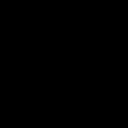
\includegraphics[scale=0.5]{imagens/black-square.png}
    \legend{Fonte:~\citeonline{tortinhas:2024}}
\end{figure}

\lipsum[1-8] % chktex-file 8


\chapter{Conclusão}%
\label{cap:conclusao}

\lipsum[1-20] % chktex-file 8

% =====

% =====
% ELEMENTOS PÓS-TEXTUAIS
% =====
\postextual{}

% --- Referências ---
\bibliography{cx_bibliografia}

% --- Glossário ---
\printglossary[type=main,style=altlist,title=Glossário]
\printglossary[type=acronym,style=altlist,title=Lista de Abreviaturas e Siglas]
% =====

\end{document}
